\newpage
\section{Arquitetura da NetFPGA}
\label{sec:arch}

Nesta seção descrevemos a arquitetura de \emph{hardware} e de
\emph{software} da NetFPGA.  Apresentamos os componentes de
\emph{hardware} presentes na NetFPGA---FPGA (\emph{field-programmable
gate array}, ou arranjo de portas programável em campo), memórias e
portas de rede---que podem ser utilizados para processar pacotes.
Também descreveremos o \emph{software} que acompanha a NetFPGA e que
serve de base para desenvolvimento de novos projetos.

\subsection{Hardware}
\label{sec:arch.hw}

O modelo clássico da NetFPGA, chamada também de NetFPGA 1G, possui
quatro portas Ethernet 1\,Gbps com processador de camada física da
Broadcom.  A NetFPGA possui um FPGA Xilinx Virtex-II Pro 50 para
processamento de pacotes, com dois núcleos PowerPC, 53.136 elementos
lógicos e ciclo de relógio de 8\,ns (125 MHz).  O FPGA é capaz de
processar pacotes recebidos pelas portas Ethernet em plena velocidade
(8\,Gbps em modo de operação \emph{full-duplex}).  A NetFPGA possui
também um controlador PCI que permite programação e comunicação com o
FPGA.

A NetFPGA possui dois bancos de memória SRAM Cypress com $2^{19}$ linhas
de 36~bits cada (espaço total de 4608\,KiB).  A SRAM pode realizar uma
operação de leitura ou escrita por ciclo de relógio e retorna dados
lidos em três ciclos de relógio.  A SRAM é ideal para aplicações que
fazem acessos frequentes a pequenas quantidades de memória, como
encaminhamento de pacotes e implementação de contadores SNMP.

A NetFPGA contém ainda dois bancos de memória DRAM Micron cada um com
$2^{24}$ linhas de 16~bits, totalizando 64\,MiB.  A DRAM funciona de
forma assíncrona e requer atualização (\emph{refreshing}) contínua dos
dados.  Por estes fatores, o controlador da DRAM é significativamente
mais complexo que o controlador da SRAM.  Apesar da maior latência, a
DRAM tem vazão alta.  A DRAM é ideal para aplicações que precisam de uma
quantidade maior de memória, como armazenamento temporário
(\emph{buffering}) de pacotes.  A DRAM também permite uma hierarquização
da memória da NetFPGA.  A Figura~\ref{fig:arch.hardware} mostra uma
visão geral da placa da NetFPGA.

\begin{figure}
\centering
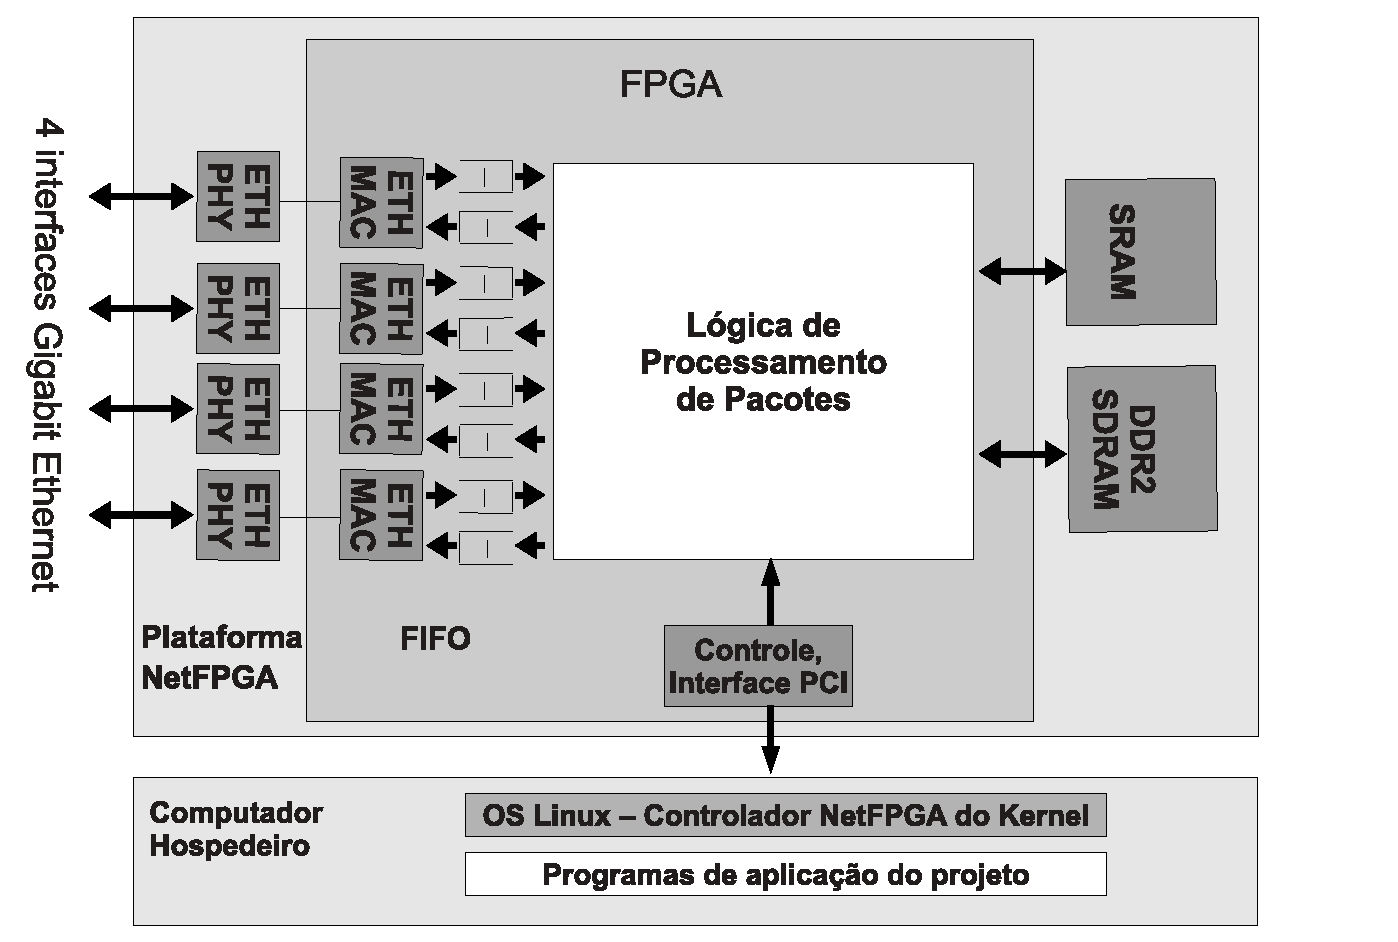
\includegraphics[scale=0.6,angle=0]{figures/placa/infraplaca.eps}
\caption{Componentes da NetFPGA.}
\label{fig:arch.hardware}
\end{figure}

A NetFPGA está disponível em outros modelos, todos com arquitetura de
\emph{hardware} similar composta de portas Ethernet, FPGA, memória SRAM
e memória DRAM.  As versões mais novas da NetFPGA suportam Ethernet
10\,Gbps, FPGAs mais velozes e memórias de maior capacidade.  Neste
material iremos nos ater à NetFPGA 1G, que serve como denominador comum
e é de mais fácil acesso.  Os conceitos e técnicas utilizados na NetFPGA
1G podem ser diretamente aplicados aos outros modelos de NetFPGA.

\subsection{Software}
\label{sec:arch.soft}

A NetFPGA possui um pacote de \emph{software} construído para facilitar
o desenvolvimento de novos projetos.  Apesar da NetFPGA permitir total
flexibilidade no processamento de pacotes, a arquitetura do
\emph{hardware} é fixa e impõe limitações.  Como é de se esperar, o
\emph{software} da NetFPGA leva a arquitetura de \emph{hardware} em
consideração e apresenta uma série de interfaces e abstrações que
utilizamos para permitir modularização e comunicação entre módulos.

\subsubsection{Projetos de referência}

A NetFPGA possui um conjunto de \emph{projetos de referência}, que a
fazem funcionar como uma placa de rede, um comutador Ethernet, ou um
roteador IP.  Nesta seção descrevemos os projetos de referência, que
servem de base para desenvolvimento de projetos mais complexos.

\subsubsection*{Placa de rede de referência}

A NetFPGA pode ser configurada como um conjunto de quatro interfaces de
rede utilizando o projeto \ssf{reference\_nic}.  Cada interface é
identificada pelo Linux como \ssf{nf2cX}, com \ssf{X} variando de
\ssf{0} a \ssf{3}.  Estas interfaces funcionam de forma análoga a
interfaces de rede como \ssf{eth0}, \ssf{wlan0}, e \ssf{lo}.

Pacotes de rede podem ser recebidos pelas interfaces \ssf{nf2cX} pela
porta Ethernet, quando outro computador envia um pacote através da rede,
ou pelo barramento PCI, quando o hospedeiro envia um pacote que deve ser
transmitido pela rede.  Para tratar o recebimento de pacotes, o
\ssf{reference\_nic} instancia oito módulos \ssf{rx\_queue} para tratar
recebimento de dados para cada interface da porta Ethernet e barramento
PCI ($4 \times 2 = 8$).  De forma análoga, o \ssf{reference\_nic}
instancia oito módulos \ssf{tx\_queue} para tratar a transmissão de
pacotes por cada interface através da porta Ethernet e barramento PCI.
Os módulos \ssf{rx\_queue} e \ssf{tx\_queue} fazem a interface entre o
FPGA, o controlador MAC e o controlador PCI.  A
\figstr~\ref{fig:arch.pipe.iface} mostra o \emph{pipeline} completo de
processamento do \ssf{reference\_nic}, com os módulos \ssf{rx\_queue} e
\ssf{tx\_queue} nas extremidades.

\begin{figure}
\centering
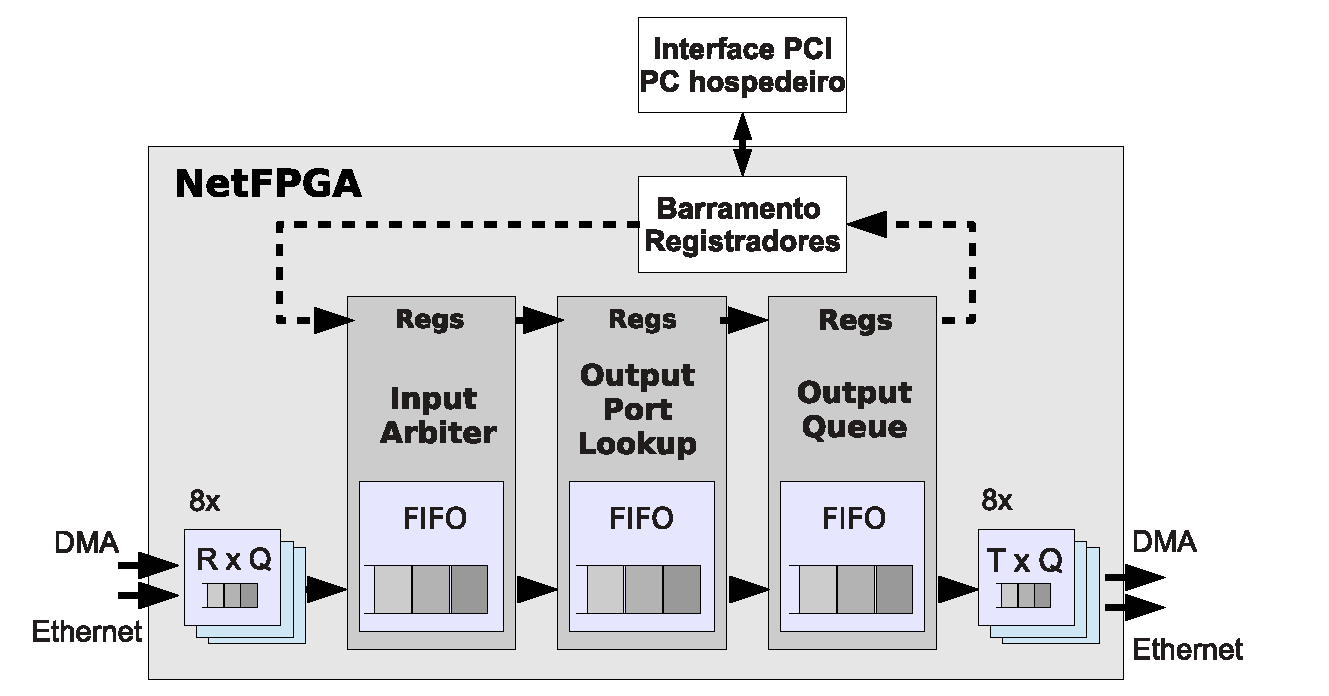
\includegraphics[scale=0.6,angle=0]{figures/modulos/datapathhor2.eps}
\caption{Pipeline de referência da NetFPGA configurada como interfaces de rede padrão.}
\label{fig:arch.pipe.iface}
\end{figure}

O processamento de pacotes na NetFPGA é realizado serialmente em um
\emph{pipeline} de múltiplos estágios.  Pacotes de rede são retirados
das filas de chegada (\ssf{rx\_queue}) pelo módulo \ssf{input\_arbiter}.
O \ssf{input\_arbiter} decide qual fila de chegada deve ser servida,
retira o pacote da fila e o coloca no \emph{pipeline} de processamento.
A política padrão de serviço é iterar sequencialmente através de todas
as filas de chegada.  Ao colocar o pacote no \emph{pipeline} de
processamento, o \ssf{input\_arbiter} adiciona um meta-cabeçalho ao
pacote indicando em qual porta ele chegou e o envia para o próximo
módulo no \emph{pipeline} de processamento.

O próximo módulo no \emph{pipeline} é o \ssf{output\_port\_lookup}, que
decide a porta de saída do pacote, adiciona essa informação no
meta-cabeçalho do pacote e o envia para o próximo módulo no
\emph{pipeline}.  A decisão da porta de saída do pacote em geral depende
dos endereços IP e MAC do destino, mas podem depender também de outras
propriedades do pacote.  Por exemplo, em nosso \emph{firewall} o destino
de pacotes TCP depende da porta de destino.  O próximo módulo no
\emph{pipeline} é o \ssf{output\_queues}, que demultiplexa o pacote do
\emph{pipeline} de processamento nas filas de saída (\ssf{tx\_queue}).

A interface de comunicação entre os módulos do \emph{pipeline} de
processamento, por exemplo como mostrado na
\figstr~\ref{fig:arch.pipe.sinais}, é padronizada.  Existem sinais
\ssf{wr} e \ssf{rdy} para controlar quando o módulo anterior está pronto
para transmitir dados e quando o módulo posterior está pronto para
receber, respectivamente.  Transmissão de dados de pacotes só acontece
quando os dois sinais estão ligados.  A interface tem ainda 8 linhas
\ssf{ctrl} que carregam sinais de controle e 64 linhas \ssf{data} que
carregam dados.  Quando \ssf{ctrl} é zero estamos transmitindo dados do
pacote. Quando \ssf{ctrl} é diferente de zero estamos transmitindo
meta-cabeçalhos do pacote.  Para cada meta-cabeçalho existe um valor de
\ssf{ctrl} pré-definido.\footnotemark{}   Desta forma, a NetFPGA
processa até 64~bits de dados de pacote por ciclo de relógio.  Dado o
ciclo de relógio de 8\,ns, o processamento de um pacote de 1500\,B leva
da ordem de 2\,$\mu$s.  A \figstr~\ref{fig:arch.pipe.sinais} ainda
mostra que módulos podem ser logicamente separados em duas partes: uma
fila para armazenamento temporário de dados e circuito para
processamento do pacote.

\footnotetext{Por exemplo, o meta-cabeçalho criado pelo
\sssf{input\_arbiter} com informações sobre a recepção de um pacote tem
\sssf{ctrl} igual a \sssf{IO\_QUEUE\_STAGE\_NUM} (\sssf{0xFF}).}

\begin{figure}
\centering
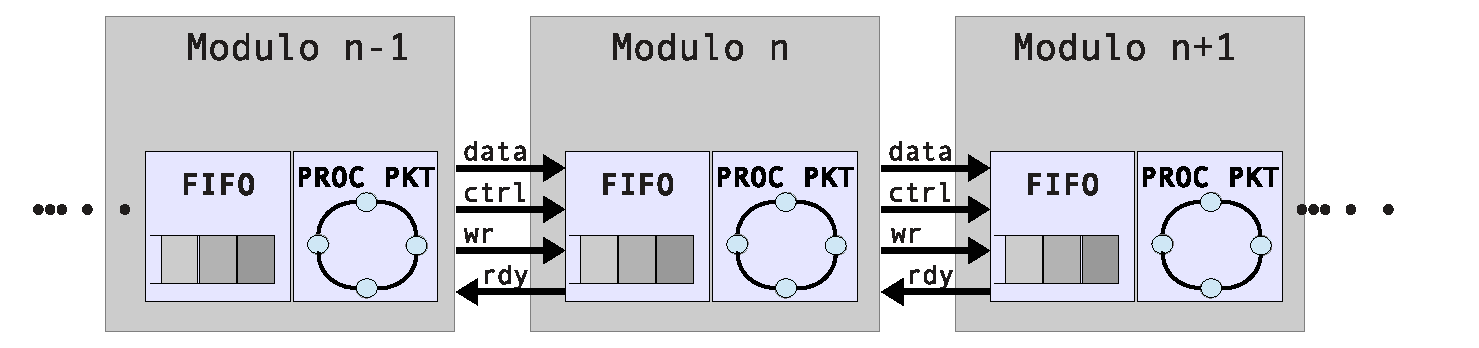
\includegraphics[scale=0.6,angle=0]{figures/modulos/fifo.eps}
\caption{Barramento de encaminhamento de pacotes.}
\label{fig:arch.pipe.sinais}
\end{figure}


\subsubsection*{Comutador de referência}

O comutador de referência (\ssf{reference\_switch}) reutiliza vários dos
módulos apresentados na descrição da placa de rede de referência.  O
único módulo com diferenças é o \ssf{output\_port\_lookup}.  No
comutador de referência, o módulo \ssf{output\_port\_lookup} associa o
endereço MAC da origem à porta Ethernet de entrada toda vez que recebe
um pacote.  Esta associação é utilizada pelo \ssf{output\_port\_lookup}
para decidir em qual porta Ethernet enviar um pacote, verificando em
qual porta o endereço MAC do destino foi observado.

\subsubsection*{Roteador de referência}

Assim como o comutador de referência, o roteador de referência
(\ssf{reference\_router}), também reutiliza vários módulos apresentados
na descrição da placa de rede de referência.  O roteador de referência
estende o módulo \ssf{output\_port\_lookup} para decidir a porta e saída
de pacotes consultando a tabela de roteamento.  A tabela de roteamento é
implementada utilizando registradores no FPGA como memória
ternária.\footnote{O módulo que implementa esta funcionalidade está
disponível em
\url{netfpga/lib/verilog/core/reference_router/cam_router}.}

Além de rotear pacotes utilizando a tabela de roteamento, o roteador de
referência precisa calcular rotas usando protocolos de roteamento como
OSPF e BGP.  Como esses protocolos são muito complexos para serem
implementados em \emph{hardware}, eles são implementados em programas
que executam no espaço do usuário.  Em outras palavras, o roteador de
referência implementa o encaminhamento de pacotes (plano de dados) em
\emph{hardware} e implementa o cálculo de rotas (plano de controle) em
\emph{software}.\footnote{O programa que implementa o plano de controle
do roteador de referência é chamado de SCONE e é armazenado em
\url{netfpga/projects/scone/}.} Como rotas precisam ser recalculadas
apenas quando há mudanças na topologia da rede, recalculá-las em
\emph{software} não compromete a latência nem a vazão do encaminhamento
de pacotes.

%\footnotetext{}

Protocolos de roteamento calculam o próximo roteador que deve ser
utilizado para encaminhar um pacote até seu destino.  O próximo roteador
no caminho é identificado pelo seu endereço IP.  Para que o roteador de
referência possa efetivamente encaminhar o pacote para o próximo
roteador, ele precisa converter o endereço IP do próximo roteador num
endereço MAC.  Esta operação é realizada pelo protocolo ARP.  O plano de
controle do roteador de referência também executa o protocolo ARP para
informar ao módulo \ssf{output\_port\_lookup} quais endereços MAC devem
ser utilizados no encaminhamento de pacotes.

\subsubsection{Estrutura de diretórios}

Para facilitar a navegação do pacote de \emph{software} da NetFPGA,
mostramos abaixo a estrutura de diretórios do pacote e uma breve
descrição do conteúdo de cada diretório.

\begin{verbnobox}[\footnotesize]
netfpga                {Diretório raiz}
   bin                 {Scripts para simulação, síntese e geração de registradores}
   bitfiles            {Diretório dos arquivos .bit dos projetos}
   lib                 {Bibliotecas de módulos e funções de simulação}
      C                {Bibliotecas C}
      java             {Biliotecas Java}
      Makefiles        {Arquivos makefile pré-definidos para simulação/síntese}
      Perl5            {Bibliotecas Perl}
      python           {Bibliotecas Python}
      release          {Arquivos XML de configuração global}
      scripts          {Scripts para configutação e testes da plataforma}
      verilog          {Módulos em Verilog para síntese}
         contributed   {Módulos Verilog de contribuidores}
         core          {Módulos Verilog oficiais}
      xml              {Arquivos XML de módulos}
   projects            {Diretório de projetos}
\end{verbnobox}

O diretório \ssf{bin} possui alguns programas de configuração do
ambiente de programação, sintetização de projetos bem como execução de
simulações e testes.  O diretório \ssf{bitfiles} contém imagens de
projetos depois de sintetizados, pontos para gravação na NetFPGA.  Como
exemplo, podemos configurar a NetFPGA com a placa de rede de referência
executando:

\begin{verbnobox}
bin/nf_download bitfiles/reference_nic.bit
\end{verbnobox}

O diretório \ssf{lib} contém o código fonte do \emph{software}.  Por
exemplo, o fonte do programa \ssf{nf\_download} é armazenado em
\ssf{netfpga/lib/C/download}.  Dentro do diretório \ssf{lib}, o
subdiretório \ssf{lib/verilog/core} armazena os módulos do núcleo da
arquitetura da NetFPGA.  Os módulos do núcleo incluem módulos como
\ssf{rx\_queue}, \ssf{tx\_queue}, \ssf{input\_arbiter},
\ssf{output\_port\_lookup}, \ssf{output\_queues} e vários outros.

A pasta \ssf{projects} contém os projetos montados pela NetFPGA.  Cada
projeto, inclusive os projetos de referência, seguem a seguinte árvore
de diretórios.

\begin{verbnobox}[\footnotesize]
   projects
      <project>        {Seu projeto}
         doc           {Documentação}
         include       {project.xml, XML de módulos criados}
         lib           {Arquivos de cabeçalho Python, Perl e C}
         src           {Módulos Verilog criados}
         sw            {Programas para teste do projeto}
         synth         {Diretório de arquivos de síntese}
         test          {Programas para testes do hardware e software em Python}
\end{verbnobox}

O diretório \ssf{doc} é utilizado para armazenar documentação do
projeto.  A pasta \ssf{include} é utilizada para armazenar os arquivos
XML de configuração; por exemplo, estes arquivos são lidos pelo programa
\ssf{nf\_register\_gen} para alocação e mapeamento dos
registradores.\footnote{O arquivo \sssf{include/project.xml} define
todos os módulos que serão instanciados no projeto, os demais arquivos
XML contém informações dos módulos implementados pelo usuário.}  A pasta
\ssf{lib} contém os cabeçalhos C, Perl e Python necessários para
utilizar os demais programas do \emph{software} da NetFPGA com este
projeto.\footnotemark{} A pasta \ssf{src} contém os módulos em Verilog
implementados pelo usuário.  Os módulos nesse diretório podem estender e
ter o mesmo nome dos módulos disponíveis em
\ssf{netfpga/lib/verilog/core}; neste caso, os módulos estendidos tem
prioridade sobre as versões originais.  As pastas \ssf{sw} e \ssf{test}
possuem programas e especificações de testes de regressão do projeto.
Por último, a pasta \ssf{synth} contém arquivos de síntese do projeto.
Iremos entrar em maiores detalhes das informações relativas a um projeto
e novos módulos Verilog na seção~\ref{sec:impl}.

\footnotetext{Um exemplo de informação nos cabeçalhos C, Perl e Python
são os identificadores de registradores.}

\subsection{Interação hardware--software}

Para facilitar a interação entre os componentes de \emph{hardware} e
\emph{software,} o projeto da NetFPGA possui algumas interfaces. Aqui
descrevemos a interface de registradores e de memória que servem para
ler e escrever dos registradores e componentes de memória,
respectivamente.

\subsubsection{Interface de registradores}
\label{sec:arch.regs}

O \emph{software} da NetFPGA define três tipos de registradores:
contadores, registradores de \emph{software} e registradores de
\emph{hardware}.  Registradores armazenam valores arbitrários.
Contadores suportam as operações de incremento, decremento, e
zerar-ao-ler (\emph{reset-on-read}).  Contadores podem ser escritos pela
NetFPGA e lidos por um programa de usuário.  Registradores de
\emph{software} podem ser escritos por programas de usuário e lidos pela
NetFPGA e registradores de \emph{hardware} são escritos pela NetFPGA e
lidos por programas de usuário.

Registradores de um módulo são definidos dentro do arquivo XML de
configuração do modulo.  O arquivo XML define as propriedades (tipo,
nome e descrição) de cada registrador do módulo.  Há nove tipos de
registradores pré-definidos no \emph{software} da NetFPGA, mais um tipo
vetor de tamanho variável, como mostrado na
tabela~\ref{tab:arch.regs.types}.


\begin{table}[h]
\centering
\begin{tabular}{lr}
\textsc{Tipo} & \textsc{Bits} \\
\ssf{ethernet\_addr}      & 48 \\
\ssf{ip\_addr}            & 32 \\
\ssf{counter32}           & 32 \\
\ssf{software32}          & 32 \\
\ssf{generic\_counter32}  & 32 \\
\ssf{generic\_hardware32} & 32 \\
\ssf{generic\_sofware32}  & 32 \\
\ssf{dataword}            & 64 \\
\ssf{ctrlword}            & 8 \\
\ssf{vetor}                     & variável \\
\end{tabular}
\caption{Tipos de registradores e exemplos de definição.}
\label{tab:arch.regs.types}
\end{table}

\newpage{}
O \emph{software} da NetFPGA provê um programa que processa os arquivos
XML de todos os módulos de um projeto, identifica os requisitos de
memória para armazenamento dos registradores de cada módulo e gera
endereços para todos os registradores do projeto.  Este programa também
gera arquivos de cabeçalho para as linguagens Verilog, C, Perl e Python
para permitir referências aos registradores do projeto bem como em
programas de usuário, simulações e testes.

\subsubsection{Interface de memória}

A NetFPGA possui dois tipos de memória: SRAM e DRAM.  A memória SRAM
executa no mesmo ciclo de relógio do FPGA e leva três ciclos para
completar acessos, mas totaliza 4.5~MiB.  A DRAM funciona de forma
assíncrona ao FPGA e leva mais ciclos de relógio para completar acessos,
mas totaliza 64~MiB.  Apesar da maior latência no acesso à DRAM, ela tem
vazão suficiente para funcionar como área de armazenamento temporário de
pacotes, por exemplo nos módulos \ssf{rx\_queue} e \ssf{tx\_queue}.

O controle do acesso à memória SRAM é realizado por um submódulo chamado
\ssf{sram\_arbiter}.  A tarefa principal do \ssf{sram\_arbiter} é
intermediar requisições de acesso à memória recebida de vários módulos e
da interface de registradores.  O \ssf{sram\_arbiter} pode ser
modificado para arbitrar o acesso à memória de diferentes formas, dando
prioridades distintas a módulos de um projeto ou para otimizar o acesso
à memória caso a aplicação tenha padrões de acessos bem definidos.
Apesar da SRAM ter tempo de acesso de três ciclos de relógio, o tempo de
acesso total através do \ssf{sram\_arbiter} depende do mecanismo de
arbitragem utilizado.  Para permitir acesso concorrente à SRAM por
diferentes módulos, o \ssf{sram\_arbiter} armazena as requisições de
acesso numa fila interna.  Detalharemos o funcionamento do
\ssf{sram\_arbiter} na seção~\ref{sec:impl.mem}.

